% 
% Annual Cognitive Science Conference
% Sample LaTeX Paper -- Proceedings Format
% 

% Original : Ashwin Ram (ashwin@cc.gatech.edu) 04/01/1994
% Modified : Johanna Moore (jmoore@cs.pitt.edu) 03/17/1995
% Modified : David Noelle (noelle@ucsd.edu) 03/15/1996
% Modified : Pat Langley (langley@cs.stanford.edu) 01/26/1997
% Latex2e corrections by Ramin Charles Nakisa 01/28/1997 
% Modified : Tina Eliassi-Rad (eliassi@cs.wisc.edu) 01/31/1998
% Modified : Trisha Yannuzzi (trisha@ircs.upenn.edu) 12/28/1999 (in process)
% Modified : Mary Ellen Foster (M.E.Foster@ed.ac.uk) 12/11/2000
% Modified : Ken Forbus 01/23/2004
% Modified : Eli M. Silk (esilk@pitt.edu) 05/24/2005
% Modified: Niels Taatgen (taatgen@cmu.edu) 10/24/2006

%% Change ``a4paper'' in the following line to ``letterpaper'' if you are
%% producing a letter-format essay.

\documentclass[10pt,letterpaper]{article}

\usepackage{cogsci}
\usepackage{pslatex}
\usepackage{apacite}
\usepackage{graphicx} %includegrahics
\usepackage{booktabs} %optimized results table
\usepackage{import}
\usepackage{amssymb} %copyright r sign
\usepackage{float}
\usepackage{verbatim} %comment

\title{Automatic Essay Grading with Latent Semantic Analysis}
 
\author{{\large \bf ZhaoBin Li
(liz2@carleton.edu)} \\
 Carleton College, 1 N. College St.
 \\
 Northfield, MN 55057 USA
 \AND {\large \bf Owen Szafran
 (szafrano@carleton.edu)} \\
 Carleton College, 1 N. College St.
 \\
 Northfield, MN 55057 USA}


\begin{document}

\maketitle

\begin{abstract}
Accurate and consistent Automated Essay Grading (AES) has been a challenge of machine learning and cognitive psychology, with interest increasing as a result of the increased usage of standardized testing in education \cite{shermis2014state}. In a meta-review on the 2012 Kaggle AES competition, Natural Language Processing through Recurrent Neural Networks, statistical analysis using Bayesian Models and Latent Semantic Analysis (LSA) were the most promising solutions implemented \cite{shermis2014state}. In this paper, we implement Generalized LSA (GLSA) on the Kaggle dataset, and investigate the ways that varying dimensions and n-gram ranges influence the accuracy of the model. Our implementation scored on average 50\% of the essays within one grade given by the human scorers. The accuracy achieved is high enough to support the idea that some semantic meaning of words can be based on contextual similarity. However, the relatively low accuracy of the model suggest that context-based similarities of words cannot fully capture the complexities of evaluating essays. We found that the optimal n-grams and dimensions are not consistent across the 8 essay questions in the dataset, yet they reveal trends that provide insight into the underlying function of GLSA. 

\textbf{Keywords:} 
Automated Essay Grading; Latent Semantic Analysis; Singular Vector Decomposition; N-Grams.
\end{abstract}

\section{Introduction}

With an increased emphasis on standardized testing, but limited resources to grade writing on standardized tests, an interest in Automated Essay Scoring (AES) has emerged \cite{shermis2014state}. A 2012 Kaggle competition showcased state-of-the-art implementations from both private corporations and research institutions and among these, three models were most prevalent among the top scoring models: Natural Language Processing using Recurrent Neural Networks, Statistical analysis using Bayesian models, and Latent Semantic Analysis \cite{shermis2014state}. Despite the common intuition that essay evaluation cannot be reduced to qualitative analysis and algorithms, the Kaggle competition demonstrated that in standardized testing, in cases where a large enough dataset is obtained, there is enough similarity across essays that computer models are able to score the essays accurately. In scoring the large-scale exams (the PARCC and SBAC) administrated to public schools across 6 US states, the top ten entries in the Kaggle competition achieved on average 98.75\% agreement with the human scores within one score point\cite{shermis2014state}. Furthermore, as the credibility of AES increases, standardized testing agencies are using commercial AES systems to assist human scores\cite{shermis2014state}. For instance, the Educational Testing Service are starting to implement the \textit{e-rater}$^{\circledR}$ to score writing sections in the prominent TOEFL iBT$^{\circledR}$ and GRE $^{\circledR}$ tests to assist human scorers \cite{ets2019aes}.

Among the available methods, we chose to implement Latent Semantic Analysis (LSA) because LSA has relatively high accuracy given its low computational demands. LSA is a statistical method which approximates the human understanding of semantic relations between words and texts by mapping them into an abstract dimensional space \cite{kintsch2002potential}. Previous literature has shown that using 300-500 dimensions emulates human perception of language, but no literature has explicitly investigated the optimal dimensionality with regards to AES \cite{kintsch2002potential}. Hence, we aim to  investigate the ways that varying the dimensionality influence the accuracy of the model. In addition, LSA is criticized for analyzing texts by counting the number of times a word appear in a text and not considering the order of the words \cite{kintsch2002potential}. Hence, to improve the accuracy of AES in scoring undergraduate essays, \citeA{islam2010automated} used n-grams as the basic element of analysis rather than words and named their method as Generalized LSA(GLSA). However, Islam and Hoque do not detail the ways in which the types of n-gram influence the model accuracy. Hence, we would like to delve into these two essential features -- dimensionality and ngram -- in the LSA algorithm in improving the accuracy of the model and providing a more in-depth look at how it functions. GLSA implemented by Islam and Hoque serves as the starting point for our own implementation. 

%\subsection{Implementation}

%For every n-gram range, we first process the training essay set and generate a n-gram-by-essay matrix. Then, we apply SVD to the matrix, extract the $U$, $S$ and $V^{T}$ components. Next, we process the validation set in the same way, and use the n-grams from the training set to generate an n-gram-by-essay matrix for the validation set. Then using the $U$, $S$ and $V^{T}$ components from the training set, we reduce the dimensionality of the training set and validation set, in order to predict the scores of the validation set. The n-gram-dimension pair which gives the greatest accuracy for predicting the scores of the validation set is then applied to the test set to get the final accuracy measure. %

\section{The LSA Method}

\subsection{Computational basis}

Dominant cognitive theories believe that people learn a word's meaning partially through its context, and thus that words which occur together in similar contexts tend to have similar meanings \cite{kintsch2002potential}. Hence, LSA aims to mimic this process by representing the connection between words and contexts as vectors in multi-dimensional space, in order to discover these similarities. Through performing a linear algebra technique called singular value decomposition (SVD) on these vectors, LSA finds contextual similarities of words and phrases, in order to analyze the semantic connections between them. SVD extracts the semantically useful features required to characterize and understand a corpus, while ignoring the noise which would disturb the data. Moreover, LSA traditionally breaks down a text into counts of individual words and loses important information about the word order. Hence, we experiment with GLSA to mitigate the information loss and achieve higher accuracy in matching the human scorers.

\begin{figure*}[ht]
\begin{center}
 \includegraphics[width=\linewidth]{img/DatasetArray.png}
\end{center}
 \caption{The Hewlett Foundation: Automated Essay Scoring dataset \cite{shermis2014state}}
\end{figure*}

\subsection{Dataset}

We obtained the dataset used in the 2012 Kaggle Competition sponsored by the Hewlett Foundation. The essays comprise responses to eight questions administered to 7th to 10th grade students in the United States. \cite{hewlett2012aes}. The details about the essay dataset are shown in figure 1 below. For every essay question, we split up the essays into training set, validation set, and test set, with 60\% of the essays being in the training set, 24\% in the validation set, and the remaining 16\% in the test set. The training set is used to generate the SVD components for every n-gram range, the validation set is used to obtain the optimal n-gram-dimensionality pair which gives the greatest accuracy measure, and then the optimal n-gram-dimensionality pair is used on the test set to obtain the final accuracy.

\subsection{Pre-processing}

We pre-process the essays to remove any distractions which are less likely to provide meaningful data about the score. These include removing commonly used words ("stopwords") and reducing the words to their base forms ("lemmatizing") \cite{islam2010automated}.

\subsubsection{n-gram Tokenization}
The main criticism of LSA is that LSA decomposes the essay into single words and does not take into account the word order \cite{kintsch2002potential}. For instance, "social network" is be seen as equivalent to "network social" in LSA. Therefore, we are inspired by Islam and Hoque to remediate the critical weakness by including n-grams and hence preserving the order of n-words, and thus implementing Generalized Latent Semantic Analysis (GLSA). By trying various n-gram start and end ranges, we aim to investigate the way these n-gram ranges influences the accuracy and improve the final accuracy measure, as well as what this tells us about the underlying function of GLSA. In the paper, we notate n-gram ranges with "(min n-gram sequence, max n-gram sequence)" - an n-gram of (1,1) means that we consider words (uni-grams) only, while an n-gram of (1, 3) means that we include uni-grams, bi-grams and tri-grams. As we are not able to pre-determine which types of n-grams are the most important, we included multiple n-grams ranges and lengths for SVD to extract the n-grams which most essentially contribute to the meanings of the essays. Ultimately, by considering groupings of words (uni-grams), phrases (tri-grams to 5-grams), and sentences (10-grams to 20-grams) rather than individual words as seen in traditional LSA, GLSA may analyze a dataset at a deeper level, and more authentically emulate human scorers. 

\subsubsection{tf-idf Weighting Scheme}

To emphasize the most salient tokens which influences the scores of the essays, we reweighted the n-gram-by-essay matrix using the term frequency–inverse essay frequency (tf-idf) weighing scheme. Tf-idf weights more heavily those terms which occur more frequently in an essay but less frequently in other essays, in order to emphasis those words more in the resulting data \cite{islam2010automated}. The equation for tf-idf is:

$$w_{i,j} = tf_{i,j} \cdot \log \frac{N}{df_i}$$

where $tf_{i,j}$ is the number of times token $i$ occurs in essay $j$ divided by the total number of tokens in $j$, $df_i$ is the number of essays containing $i$ and $N$ is the total number of essays.

Initially, the weight of an n-gram in the essay is the count of the number of times a token appears in the essay which may not be an accuracy measure. However, when we tried weighting by count only for the first essay question, 'computer' and 'people' appears the most frequently across all the essays. With the addition of tf-idf weighting, the model will take into account these two words much less, since these two words are not useful in distinguishing between the essays. However, after applying tf-idf, the weights of these two words decreases significantly and the accuracy measure increases by around 10-20\%. Therefore, tf-idf emphasizes the more unique features characterizing the scores of the essays to help SVD extract the more important latent features.

\subsection{Singular Value Decomposition}

We applied SVD on the n-gram-by-essay matrix to extract the most important dimensions ("latent features") characterizing the scores of the essays. Through SVD, we eliminated redundant information ("noise") and enriched the similarity data of the n-gram vectors between essays, as measured by cosine similarity. In the context of decomposing a $W$ re-weighted n-grams by $D$ essays matrix X, we can express the product as follows \cite{islam2010automated}: 

$$X_{W\times D} = U_{W\times D} \times S_{D \times D} \times V^{T}_{D \times D}$$

\begin{figure}[H]
\begin{center}
\includegraphics[width=\linewidth]{img/SVD.eps}
\end{center}
\caption{Singular Vector Decomposition \cite{islam2010automated}} 
\end{figure}

Where $S$ is a diagonal matrix with singular values, which corresponds to the importance of every n-gram token for determining the contextual similarity between essays, arranged in ascending order.

To eliminate the less important n-grams and extract the most important semantic characteristics in the essay dataset, SVD truncates the smaller singular values together with the corresponding columns and rows of $U$ and $V^T$. Upon reducing the dimensionality of the training set matrix $S$ to a chosen dimensionality $d$, we get a new $W \times D$ matrix $Z$ with the original dimensions, which is \cite{islam2010automated}:
$$Z_{W\times D} = U_{W\times d} \times S_{d \times d} \times V^{T}_{d \times D}$$

\begin{figure}[H]
\begin{center}
\includegraphics[width=\linewidth]{img/SVDReduced.eps}
\end{center}
\caption{Singular Vector Decomposition with dimensionality reduction \cite{islam2010automated}} 
\end{figure}

\subsection{Comparing Essays}

To enable comparison between the training set, the validation and test set, once we have reduced the dimensionality of all three sets using the $U$ and $S$ components of the SVD, we want this matrix in essays-by-dimension space, rather than words-by-essay space, so that we can compare the essays at the specified dimensionality. We obtain this reduced matrix $Z'_{D\times d}$ for the training set by multiplying the transpose of the original matrix by the principle components $U_{W\times d}$ and $ S^{-1}_{d \times d}$, as shown below \cite{islam2010automated}:

$$Z'_{D\times d} = X^T_{D\times W} \times U_{W\times d} \times S^{-1}_{d \times d}$$

Then using the n-grams from the training set, we construct an n-gram-by-essay matrix for the validation set and test set, and apply the same SVD transformation on a new essay set, used either for validation or testing purposes, $k_{V \times W}$ to obtain the reduced matrix $k'_{V \times d}$, where $V$ is the number of essays in the validation or test set set. \cite{islam2010automated}:

$$k'_{V \times d} = k^T_{V \times W} \times U_{W\times d} \times S^{-1}_{d \times d}$$

\subsubsection{Assigning scores using Cosine Similarity}
In these matrices, each row represents an essay, so we can then compare each pair of essays between the reduced essay vectors in the training set $Z'_{D\times d}$ and the reduced essay vectors in the validation set $k'_{V \times d}$, by finding the cosine similarity of each pair of rows. 

To enable comparison across essay question, we scaled the essay scores for every question to between 1 and 10 using a min-max scalar. We assigned the scores for every essay in the validation set and the test set by comparing the cosine similarity between the essay and every essay in the training set \cite{islam2010automated}. Cosine Similarity is defined as:

$$cos(x, y) = \frac {x \cdot y}{||x|| \cdot ||y||}$$

where $x$ refers to the transformed essay in the validation or test set that we seek to score, and $y$ refers to the essay in the training set with labelled scores \cite{islam2010automated}. A grade is assigned for a given essay in the validation set by choosing the grade of the most similar essay in the training set.

\subsection{Measuring accuracy using the F1 score}

We uses a weighted F1 score which takes into account the number of false positives (precision) and false negative (recall) besides the correctly assigned scores (the true positive) to give a more nuanced measure of the actual effectiveness of the model \cite{islam2010automated}: 

$$\mathrm{Precision_i} = \frac {\textrm{No. of essays correctly assigned score } i} {\textrm{Total No. of essays Model assigned score } i}$$
$$\mathrm{Recall_i} = \frac{\textrm{No. of essays correctly assigned the score } i}{\textrm{No. of essays actually graded score } i}$$
$$\mathrm{F1_i} = \frac{\mathrm{2 \cdot \mathrm{Precision_i} \cdot \mathrm{Recall_i}}}{\mathrm{Precision_i + Recall_i}}$$
$$\mathrm{F1} = \sum_{i=0}^{10} \mathrm{F1_i} \cdot \frac{\textrm{No. of essays graded score } i} {\textrm{Total no. of essays}}$$


Initially, we used the simple accuracy measure for the number of essays the model assigned the correct score. However, we realized that when score variation is low, the models which assign all essays a similar score has the chance to score the highest in accuracy. For instance, for essay question one, the the n-gram range of (10, 20) assigned the most percentage of essays with the correct score. Upon close inspection, we saw that the variation of the labelled score is low, and most is around 7, and an n-gram range of (10, 20) which takes into account sequences of sentences and beyond does not distinguish between the essays well and assign almost all scores to be 7. However, we do not consider the LSA model to have learned the key features of a high scoring essay as opposed to a low scoring essay. However, the F1 score will take into account the high number of false positives of the model and hence give the model a low F1 score score. Hence using the F1 score is a better reflection of accuracy than the percentage of essays with the correct score. 

\subsection{Optimizing n-grams and dimensionality}

For every essay question, we split the essay into training, validation and test sets. We used the training set to get the SVD components for every n-gram range. Then, we experimented to find the optimal dimension $d_{optimal}$ which gives the greatest accuracy. To do so, we tested various dimensions between 0 to approximately 1000 to reduce the training and validation set. For every dimension, we then assign the score for the validation set by comparing the similarities between the essays in the training and validation set. The n-gram and dimension pair which give the greatest F1 score on the validation set is then chosen to apply on the test set. The F1 score obtained from the test set is taken as the final accuracy. 

\section{Results}

\subsubsection{Finding the optimal Dimensionality}

For each n-gram range, we sought out the optimal dimension, which gives the greatest F1 score in the validation set. For 30 dimensions spread evenly between 0 (the minimum possible dimensions) and the number of essays in the training set (the maximum possible dimensions), we obtained the F1 score and plotted them in the graph below, shown here for question 1, plotted in the Figure \ref{Q1Ngram5to15}.

\begin{figure}[ht]
\begin{center}
\includegraphics[width=\linewidth]{img/Q1Ngram5to15.eps}
\end{center}
\caption{F1 Score Across dimensions for Question 1, n-gram (5,15)}
\label{Q1Ngram5to15}
\end{figure}

For question 1, we see that, for n-gram range (5, 15) the optimal dimension is at 921 in the validation set. For every n-gram range, we perform the same process and the resulting function of F1 scores versus dimensions, for each n-gram range, is plotted in the Figure \ref{Q1F1ByNgramsAcrossDimensions}.

\begin{figure}[ht]
\begin{center}
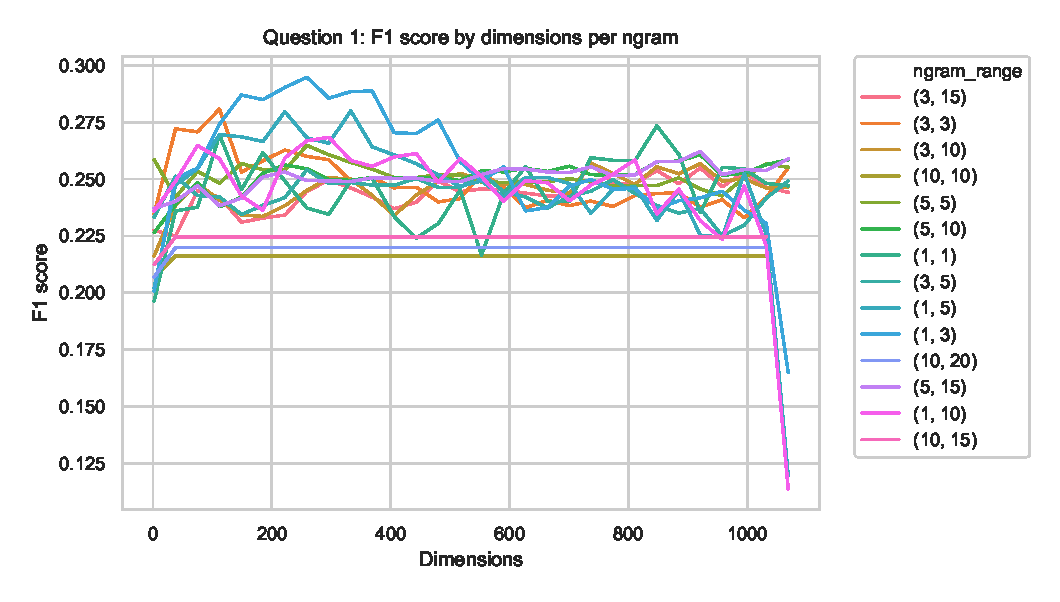
\includegraphics[width=\linewidth]{img/Q1F1ByNgramsAcrossDimensions.eps}
\end{center}
\caption{F1 Score Across dimensions for Question 1}
\label{Q1F1ByNgramsAcrossDimensions}
\end{figure}

We used this data to find the optimal dimension for each n-gram range, which are used later in determining the optimal n-gram for each question. We repeat this process across each question, so that we have the optimal dimensionality data for every n-gram range, on each question. For question 1, the optimal n-gram range is (5, 15) at dimension 921, as shown in Figure \ref{Q1OptimumDimensions}.

\begin{figure}[ht]
\begin{center}
\includegraphics[width=\linewidth]{img/Q1OptimumDimensions.eps}
\end{center}
\caption{Optimum dimensions for all n-gram ranges in Question 1}
\label{Q1OptimumDimensions}
\end{figure}

\subsubsection{Analysis}
The graph of F1 scores against dimensions for every n-gram in Question 1, shown in Figure 5, reveals a general trend which explains the role of dimension reduction in LSA. Generally, across all n-grams, the F1 scores start low, and then increase, remain relatively constant and then sharply decrease. At lower dimensions, adding more dimensions captures more useful semantic features to determine the similarities more accurately. Thereafter at higher dimensions, adding more dimensions captures more noise and results in the sharp decrease in F1 score. Another trend we observed in Figure 6 is that ngram-ranges which are wider (larger max n-gram $-$ min ngram value) have higher optimal dimensions. We believe that a wider ngram-range include more semantically meaningful n-gram tokens and thereby cannot be reduced to lower dimensions.

We similarly plotted the optimal dimensions, for the optimal n-grams, across all the questions to further investigate the impact of dimensionality reduction in LSA in Figure \ref{OptimumDimensions}.

\begin{figure}[ht]
\begin{center}
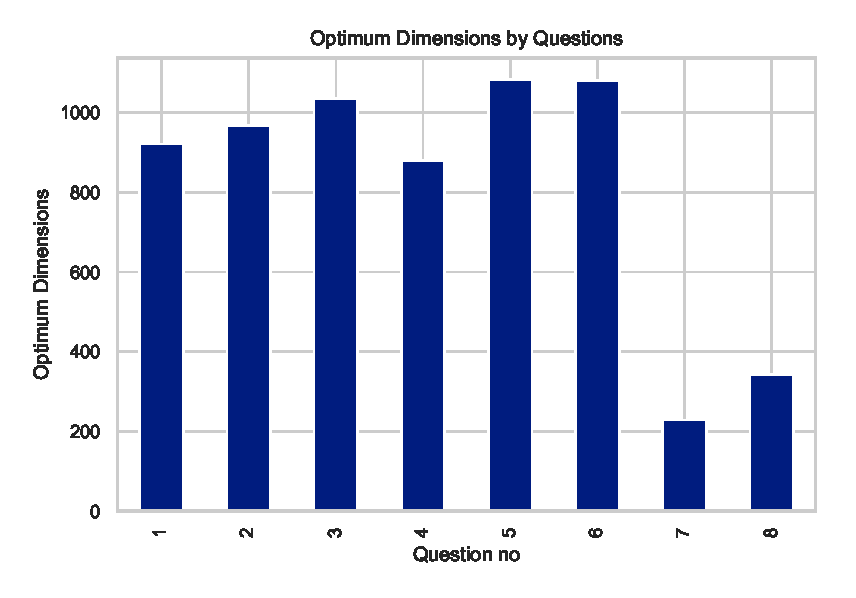
\includegraphics[width=\linewidth]{img/OptimumDimensions.eps}
\end{center}
\caption{Optimal Dimensions by Question}
\label{OptimumDimensions}
\end{figure}

For questions 1 to 6, we found that the optimum dimensionality was between 800 and 1000. We attribute the relatively high optimal dimensions to the essays having been written by 8th and 10th graders, who have more extensive vocabulary. Thus, more dimensions are necessary to capture the important features of the essays and grade the essays accurately. In contrast, questions 7 and 8 have optimal dimensions in between 200 and 400. We are able to explain the low dimensions for question 8 but not 7.  Question 8 has only 918 essays, which is roughly half the number of essays compared to all the other questions. As there are less essays, less dimensions may be necessary to capture the important features within them. Initially, we speculated that question 7 is the only question written by 7th graders, which likely means that the vocabulary used is relatively limited, making the data less complex. Hence, there are less unique sets of words used and less dimensions are required to characterize them. However, a  count of unique words shows that question 7 has around 7000 words, which is twice that of question 4, 5 and 5 at over 3000 words each.

\subsubsection{Finding the Optimal n-grams}For every n-gram, we found the optimal dimensions that give the greatest F1 score for the validation set. We then use the same n-grams to generate the n-gram-by-essay matrix for the test set and reduced the test set to the same optimal dimension. We then assigned scores to the test set and obtained F1 scores for the optimal dimension for every n-gram range. The dimensionality-n-gram pair which gives the greatest F1 score on the test set is then chosen to generate the final F1 score, and these scores are shown in figure 11.

To illustrate the process for question 1, we plotted the F1 score for the optimal dimension for every n-gram range below in Figure \ref{Q1F1ByNgrams}

\begin{figure}[ht]
\begin{center}
\includegraphics[width=\linewidth]{img/Q1F1ByNgrams.eps}
\end{center}
\caption{Question 1 F1 Score for each n-gram}
\label{Q1F1ByNgrams}
\end{figure}

We then repeated the process across all the question to obtain the optimal n-gram-dimensionality pairs for each question, in order to get the final F1 score, shown in Figure \ref{F1ByQuestions}.


\subsubsection{Analysis}
To better analyze why certain n-gram ranges are optimal for certain questions, we plotted the optimum F1 scores for all the questions (noting the the n-gram ranges below every question) in Figure \ref{F1ByQuestions}.

\begin{figure}[ht]
\begin{center}
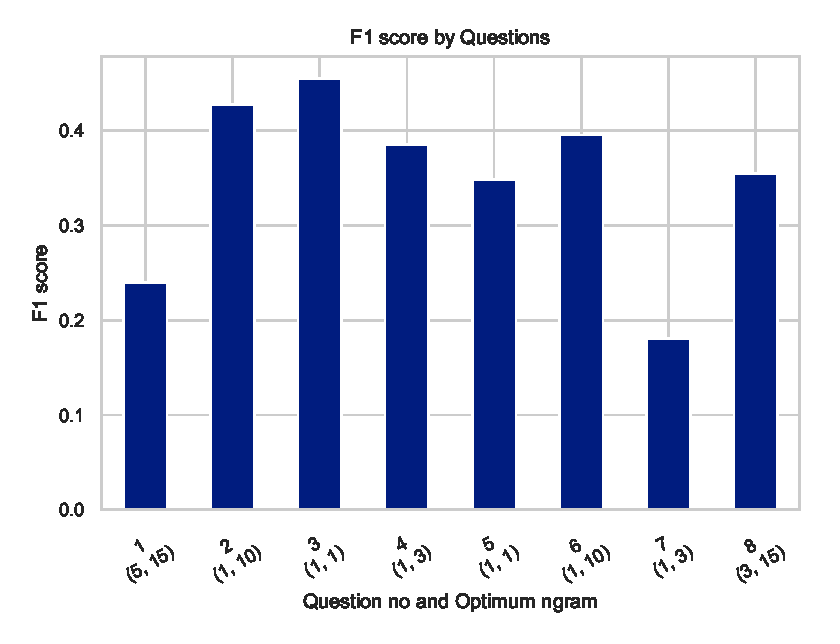
\includegraphics[width=\linewidth]{img/F1ByQuestions.eps}
\end{center}
\caption{Optimum F1 Score by Question, Ngram}
\label{F1ByQuestions}
\end{figure}

\subsubsection{Longer n-gram ranges correspond to longer essays}
As we see in Figure \ref{F1ByQuestions}, there is a wide range of optimal n-gram ranges for the 8 questions. The general trend is that the minimum and maximum n-gram is low: for 6 questions, the optimal n-grams start at 1 and for 4 questions the optimal n-grams end at less than 3. Questions 1 and 8 are the only questions to have 15 as the maximum n-gram. In addition, question 8's minimum n-gram is 3, and question 1's is 5. As question 8 has a mean length of responses at 622.1 which is significantly longer than all the other questions, as shown in figure 1, the essay comprises more sentences and the order of sentences ought to influence the score. Hence, we speculate that a longer n-gram of 15 (roughly equivalent to 2 sentences, totaling 104786 in question 8) is required to capture the order of sentences. Our explanation is further supported by the data which shows that questions 1 and 2, the next two longest essays, have the next two greatest n-gram ranges of (5,15) and (1,10) respectively. In contrast, Questions 3, 4, and 5, contain the shortest sets of essays and have the shortest optimal n-gram ranges. For shorter essays, shorter n-grams are more relevant for determining the score.

We also realize that in general for essays with higher maximum n-grams, the minimum n-grams is also greater. Longer n-grams become more effective at characterizing the important semantic features of the essays. Thus, shorter n-grams correlate less to the meaning of the essay as a whole and their roles in providing meaningful data decrease and hence are not included in the optimum n-gram range. 

\subsubsection{Longer n-gram ranges correspond to more complex essays}
Another interesting case is the stark contrast in optimum n-gram ranges between questions 6 and 7. While both essays are of similar lengths at 153.64 words and 171.28 words, respectively, question 6 has an optimal n-gram range of (1,10) whereas question 7 has the optimal of (1,3). We believe the contrast is because question 6's responses were written by 10th grade students, while question 7's responses were written by 7th grade students. It stands to reason that, although both have middle essay lengths, responses to question 7 most likely comprise much shorter, simpler sentences than question 6 and hence require shorter n-grams to capture the meaning of these sentences.

\section{Discussion}
Our results provided several insights into the function and usefulness of LSA. Our accuracy, F1 Score, and Absolute Error are  in Table \ref{OptRes}:

\begin{table}[h]
\centering
\subimport{data/}{optimized_results.tex}
\caption{Overview of Model Accuracy}
\label{OptRes}
\end{table}

\subsubsection{Accuracy Discussion}

In the table above, accuracy is the measure of questions that were within one grade of the actual score, and absolute error is the measure of the difference between the model-predicted score and the actual score. We have a wide range of accuracy: for questions 1 and 8, the accuracy is 62\% and 75\% respectively. These, as discussed above, are the questions with the greatest n-gram ranges. However, for the other questions, our accuracy varies from 35\% to 46\%. Since we counted predictions within one score as correct, random guesses would be approximately 30\% correct. Thus, for the majority of the questions, we have low accuracy, with only a slight improvement over random chance. These show us that LSA reasonably captures the semantic features of writing for longer essays through the use of longer n-grams, but does not do so effectively for shorter, less-complex essays. Based on our best knowledge, no research has come to our conclusion as yet.

Additionally, the F1 score for a random chance model would be approximately .1, and our F1 scores, with an average of 0.348, are generally well above the random average. However they are not high enough to support the claim that GLSA is a consistent, precise, and accurate model for AES. Lastly, the absolute error ranges from 0.957 to 2.493, showing that on some questions the model gives generally accurate scores but not on others. The range of absolute error show that although some aspects of semantics are derived from contextual similarity, resulting in LSA performing better than random, context-based similarity alone does not fully capture the complexities of writing, nor fully address the problem of Automated Essay Grading. 


\subsubsection{Further Work}
As discussed in the accuracy section above, our results suggest the possibility that GLSA would be more efficient with longer essays. We may attempt a similar process on a dataset of longer responses to check if GLSA may increase in accuracy and F1 score. In addition, approaches using Recurrent Neural Networks and Bayesian models could be directly compared to GLSA to analyze the different aspects of the data they focus on. Lastly, investigating the possibility of combining certain aspects of GLSA with other models could also be an interesting extension.

\bibliographystyle{apacite}

\setlength{\bibleftmargin}{.125in}
\setlength{\bibindent}{-\bibleftmargin}

\bibliography{CogSci_Template}

\end{document}
